\PassOptionsToPackage{unicode=true}{hyperref} % options for packages loaded elsewhere
\PassOptionsToPackage{hyphens}{url}
%
\documentclass[ignorenonframetext,]{beamer}
\usepackage{pgfpages}
\setbeamertemplate{caption}[numbered]
\setbeamertemplate{caption label separator}{: }
\setbeamercolor{caption name}{fg=normal text.fg}
\beamertemplatenavigationsymbolsempty
% Prevent slide breaks in the middle of a paragraph:
\widowpenalties 1 10000
\raggedbottom
\setbeamertemplate{part page}{
\centering
\begin{beamercolorbox}[sep=16pt,center]{part title}
  \usebeamerfont{part title}\insertpart\par
\end{beamercolorbox}
}
\setbeamertemplate{section page}{
\centering
\begin{beamercolorbox}[sep=12pt,center]{part title}
  \usebeamerfont{section title}\insertsection\par
\end{beamercolorbox}
}
\setbeamertemplate{subsection page}{
\centering
\begin{beamercolorbox}[sep=8pt,center]{part title}
  \usebeamerfont{subsection title}\insertsubsection\par
\end{beamercolorbox}
}
\AtBeginPart{
  \frame{\partpage}
}
\AtBeginSection{
  \ifbibliography
  \else
    \frame{\sectionpage}
  \fi
}
\AtBeginSubsection{
  \frame{\subsectionpage}
}
\usepackage{lmodern}
\usepackage{amssymb,amsmath}
\usepackage{ifxetex,ifluatex}
\usepackage{fixltx2e} % provides \textsubscript
\ifnum 0\ifxetex 1\fi\ifluatex 1\fi=0 % if pdftex
  \usepackage[T1]{fontenc}
  \usepackage[utf8]{inputenc}
  \usepackage{textcomp} % provides euro and other symbols
\else % if luatex or xelatex
  \usepackage{unicode-math}
  \defaultfontfeatures{Ligatures=TeX,Scale=MatchLowercase}
\fi
% use upquote if available, for straight quotes in verbatim environments
\IfFileExists{upquote.sty}{\usepackage{upquote}}{}
% use microtype if available
\IfFileExists{microtype.sty}{%
\usepackage[]{microtype}
\UseMicrotypeSet[protrusion]{basicmath} % disable protrusion for tt fonts
}{}
\IfFileExists{parskip.sty}{%
\usepackage{parskip}
}{% else
\setlength{\parindent}{0pt}
\setlength{\parskip}{6pt plus 2pt minus 1pt}
}
\usepackage{hyperref}
\hypersetup{
            pdftitle={Dynamic Documents using R: Hands-On},
            pdfborder={0 0 0},
            breaklinks=true}
\urlstyle{same}  % don't use monospace font for urls
\newif\ifbibliography
\usepackage{color}
\usepackage{fancyvrb}
\newcommand{\VerbBar}{|}
\newcommand{\VERB}{\Verb[commandchars=\\\{\}]}
\DefineVerbatimEnvironment{Highlighting}{Verbatim}{commandchars=\\\{\}}
% Add ',fontsize=\small' for more characters per line
\usepackage{framed}
\definecolor{shadecolor}{RGB}{248,248,248}
\newenvironment{Shaded}{\begin{snugshade}}{\end{snugshade}}
\newcommand{\AlertTok}[1]{\textcolor[rgb]{0.94,0.16,0.16}{#1}}
\newcommand{\AnnotationTok}[1]{\textcolor[rgb]{0.56,0.35,0.01}{\textbf{\textit{#1}}}}
\newcommand{\AttributeTok}[1]{\textcolor[rgb]{0.77,0.63,0.00}{#1}}
\newcommand{\BaseNTok}[1]{\textcolor[rgb]{0.00,0.00,0.81}{#1}}
\newcommand{\BuiltInTok}[1]{#1}
\newcommand{\CharTok}[1]{\textcolor[rgb]{0.31,0.60,0.02}{#1}}
\newcommand{\CommentTok}[1]{\textcolor[rgb]{0.56,0.35,0.01}{\textit{#1}}}
\newcommand{\CommentVarTok}[1]{\textcolor[rgb]{0.56,0.35,0.01}{\textbf{\textit{#1}}}}
\newcommand{\ConstantTok}[1]{\textcolor[rgb]{0.00,0.00,0.00}{#1}}
\newcommand{\ControlFlowTok}[1]{\textcolor[rgb]{0.13,0.29,0.53}{\textbf{#1}}}
\newcommand{\DataTypeTok}[1]{\textcolor[rgb]{0.13,0.29,0.53}{#1}}
\newcommand{\DecValTok}[1]{\textcolor[rgb]{0.00,0.00,0.81}{#1}}
\newcommand{\DocumentationTok}[1]{\textcolor[rgb]{0.56,0.35,0.01}{\textbf{\textit{#1}}}}
\newcommand{\ErrorTok}[1]{\textcolor[rgb]{0.64,0.00,0.00}{\textbf{#1}}}
\newcommand{\ExtensionTok}[1]{#1}
\newcommand{\FloatTok}[1]{\textcolor[rgb]{0.00,0.00,0.81}{#1}}
\newcommand{\FunctionTok}[1]{\textcolor[rgb]{0.00,0.00,0.00}{#1}}
\newcommand{\ImportTok}[1]{#1}
\newcommand{\InformationTok}[1]{\textcolor[rgb]{0.56,0.35,0.01}{\textbf{\textit{#1}}}}
\newcommand{\KeywordTok}[1]{\textcolor[rgb]{0.13,0.29,0.53}{\textbf{#1}}}
\newcommand{\NormalTok}[1]{#1}
\newcommand{\OperatorTok}[1]{\textcolor[rgb]{0.81,0.36,0.00}{\textbf{#1}}}
\newcommand{\OtherTok}[1]{\textcolor[rgb]{0.56,0.35,0.01}{#1}}
\newcommand{\PreprocessorTok}[1]{\textcolor[rgb]{0.56,0.35,0.01}{\textit{#1}}}
\newcommand{\RegionMarkerTok}[1]{#1}
\newcommand{\SpecialCharTok}[1]{\textcolor[rgb]{0.00,0.00,0.00}{#1}}
\newcommand{\SpecialStringTok}[1]{\textcolor[rgb]{0.31,0.60,0.02}{#1}}
\newcommand{\StringTok}[1]{\textcolor[rgb]{0.31,0.60,0.02}{#1}}
\newcommand{\VariableTok}[1]{\textcolor[rgb]{0.00,0.00,0.00}{#1}}
\newcommand{\VerbatimStringTok}[1]{\textcolor[rgb]{0.31,0.60,0.02}{#1}}
\newcommand{\WarningTok}[1]{\textcolor[rgb]{0.56,0.35,0.01}{\textbf{\textit{#1}}}}
\usepackage{graphicx,grffile}
\makeatletter
\def\maxwidth{\ifdim\Gin@nat@width>\linewidth\linewidth\else\Gin@nat@width\fi}
\def\maxheight{\ifdim\Gin@nat@height>\textheight\textheight\else\Gin@nat@height\fi}
\makeatother
% Scale images if necessary, so that they will not overflow the page
% margins by default, and it is still possible to overwrite the defaults
% using explicit options in \includegraphics[width, height, ...]{}
\setkeys{Gin}{width=\maxwidth,height=\maxheight,keepaspectratio}
\setlength{\emergencystretch}{3em}  % prevent overfull lines
\providecommand{\tightlist}{%
  \setlength{\itemsep}{0pt}\setlength{\parskip}{0pt}}
\setcounter{secnumdepth}{0}

% set default figure placement to htbp
\makeatletter
\def\fps@figure{htbp}
\makeatother

\hypersetup{colorlinks, linkcolor=, urlcolor=blue, citecolor=blue}

\title{Dynamic Documents using R: Hands-On}
\author{Fernando Hoces de la Guardia\\
BITSS\\
-\\
Slides at\\
\hspace*{0.333em}\url{https://github.com/BITSS/CEGA2019}}
\date{CEGA, October 2019}

\begin{document}
\frame{\titlepage}

\begin{frame}
\tableofcontents[hideallsubsections]
\end{frame}
\hypertarget{dynamic-documents-for-computational-reproducibility}{%
\section{Dynamic Documents For Computational
Reproducibility}\label{dynamic-documents-for-computational-reproducibility}}

\begin{frame}[fragile]{Dynamic Documents For Computational
Reproducibility}
\protect\hypertarget{dynamic-documents-for-computational-reproducibility-1}{}

\begin{itemize}
\tightlist
\item
  Based on principles of \emph{literate programming} aims at combining
  code and paper in one single document
\item
  Best framework to achieve the holy grail of \textbf{one-click
  reproducible workflow}
\item
  Best two current implementations: \texttt{RMarkdown\ (R)} \&
  \texttt{Jupyter\ (Python)}. \texttt{Stata} is catching up (dyndocs
  release \href{https://www.stata.com/new-in-stata/markdown/}{here} and
  reviews
  \href{http://data.princeton.edu/stata/markdown/markstat.htm}{here} and
  \href{https://www.bitss.org/2017/09/05/review-of-statas-dyndoc/}{here})
\end{itemize}

\end{frame}

\begin{frame}{Currently code and narrative components live in separate
universes}
\protect\hypertarget{currently-code-and-narrative-components-live-in-separate-universes}{}

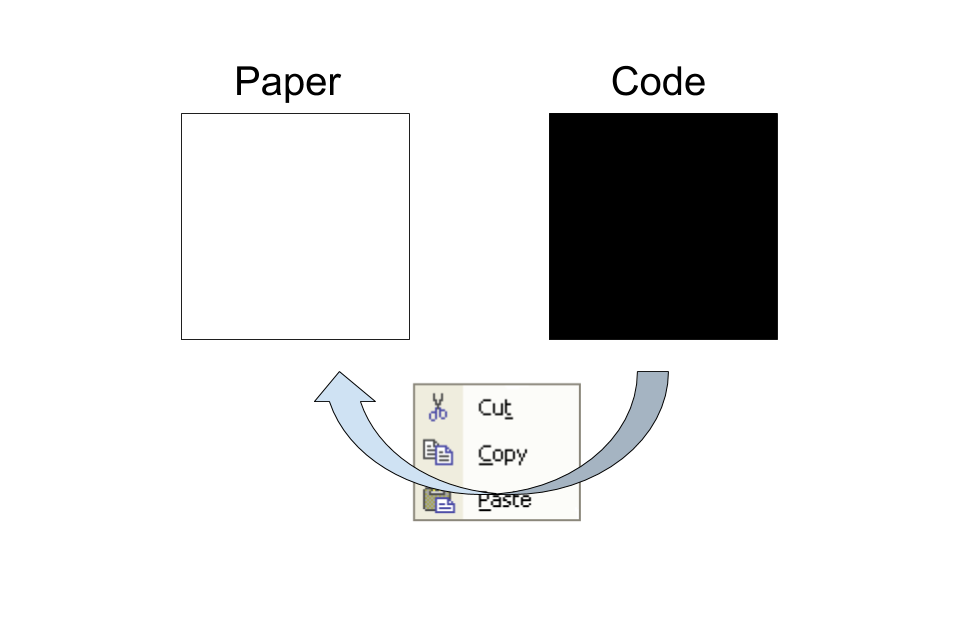
\includegraphics{../Images/Two universes.png}

\end{frame}

\begin{frame}{Dynamic Documents: integrate the two universes!}
\protect\hypertarget{dynamic-documents-integrate-the-two-universes}{}


\includegraphics{../Images/One universe.png}

\end{frame}

\begin{frame}[fragile]{Dynamic Documents: A Recipe}
\protect\hypertarget{dynamic-documents-a-recipe}{}

\begin{itemize}
\tightlist
\item
  1 simple language that can combine text and code: \texttt{Markdown}
\item
  1 statistical package to do the analysis (\texttt{R}, \texttt{Python},
  \texttt{3S\textquotesingle{}s?})
\item
  1 machinery to combine analysis and text to create a single output:
  \texttt{Pandoc}
\item
  {[}Optional-but-not-really{]} 1 program to bring all the elements
  together: RStudio/RMarkdown, Jupyter
\end{itemize}

\end{frame}

\begin{frame}{Markdown laguange/syntax in 60 seconds}
\protect\hypertarget{markdown-laguangesyntax-in-60-seconds}{}

\includegraphics{../Images/RStudioCS.png}

\end{frame}

\hypertarget{one-type-of-dynamic-document-r-markdown}{%
\section{One Type of Dynamic Document: R
Markdown}\label{one-type-of-dynamic-document-r-markdown}}

\begin{frame}[fragile]{For our excercise: R Markdown}
\protect\hypertarget{for-our-excercise-r-markdown}{}

\begin{itemize}
\tightlist
\item
  \texttt{R}: \textbf{open source} programming language design for
  statistical analysis.\\
\item
  RStudio: free software that provides and Integrated Development
  Environment (IDE)\\
\item
  RStudio combines all together: R + Markdown + Pandoc to produce
  multiple outputs 
\includegraphics{../Images/RMarkdownFlow.png}
\end{itemize}

\end{frame}

\begin{frame}{R Markdown}
\protect\hypertarget{r-markdown}{}


\includegraphics[width=0.8\textwidth,height=\textheight]{../Images/RMarkdownOutputFormats.png}

\end{frame}

\begin{frame}{Basic Structure}
\protect\hypertarget{basic-structure}{}

\begin{itemize}
\tightlist
\item
  A header
\item
  Text
\item
  Code: inline and chunks
\end{itemize}

\end{frame}

\begin{frame}[fragile]{Basic Structure: Header}
\protect\hypertarget{basic-structure-header}{}

\begin{Shaded}
\begin{Highlighting}[]
\OperatorTok{---}
\NormalTok{title}\OperatorTok{:}\StringTok{ "Sample Paper"}
\NormalTok{author}\OperatorTok{:}\StringTok{ "Fernando Hoces de la Guardia"}
\NormalTok{output}\OperatorTok{:}\StringTok{ }\NormalTok{html_document}
\OperatorTok{---}
\end{Highlighting}
\end{Shaded}

\end{frame}

\begin{frame}[fragile]{Basic Structure: Body of Text}
\protect\hypertarget{basic-structure-body-of-text}{}

\begin{Shaded}
\begin{Highlighting}[]
\OperatorTok{---}
\NormalTok{header}
\OperatorTok{---}
\end{Highlighting}
\end{Shaded}

This is where you write your paper. Nothing much to add. You can check
Markdown
\href{https://www.rstudio.com/wp-content/uploads/2015/02/rmarkdown-cheatsheet.pdf}{syntax
here}. And it can use can type equations using LaTex syntax!

\end{frame}

\begin{frame}[fragile]{Basic Structure: Code Chunks and Inline}
\protect\hypertarget{basic-structure-code-chunks-and-inline}{}

\begin{Shaded}
\begin{Highlighting}[]
\OperatorTok{---}
\NormalTok{header}
\OperatorTok{---}
\end{Highlighting}
\end{Shaded}

Body of text.

To begin a piece of code (``code chunk''). Enclose them in the following
expression (Ctrl/Cmd + shift/optn + i)

\begin{verbatim}
```{r, eval=TRUE}
here goes the code
```
\end{verbatim}

To write inline use only one Back-tick to open followed by an ``r'' and
one to close \texttt{\textasciigrave{}r\ 1+1\textasciigrave{}} in the
output.

\end{frame}

\hypertarget{practical-excercise-1}{%
\section{Practical Excercise \#1}\label{practical-excercise-1}}

\begin{frame}{Goals for excercise \#1}
\protect\hypertarget{goals-for-excercise-1}{}

\textbf{Primary Goals:}\\
1 - Become familiar with your first DD.\\
2 - Compile an empty (or default) DD into multiple formats.\\
3 - Edit a DD with some narrative, some code (in R) and some math
(optional).\\
4 - Present all the results dynamically into multiple outputs.

\pause

\textbf{Secondary Goal:}\\
1 - Expose you to some R programming.\\
2 - Entertain you with a fun problem.

\end{frame}

\begin{frame}{Hands-on excercise: the birthday problem!}
\protect\hypertarget{hands-on-excercise-the-birthday-problem}{}

As an illustration lets write a report using the participants in this
workshop to illustrate the famous
\href{https://en.wikipedia.org/wiki/Birthday_problem}{birthday problem}.

\begin{quote}
What is the probability that at least two people this room share the
same birthday?
\end{quote}

\begin{quote}
There are 23 in this room.
\end{quote}

\begin{quote}
Is it something like \(\frac{1}{365} \times 23=\) 0.063?
\end{quote}

\end{frame}

\begin{frame}[fragile]{Create a new RMarkdown File}
\protect\hypertarget{create-a-new-rmarkdown-file}{}

1 - In RStudio:
\texttt{File-\textgreater{}\ New\ File\ -\textgreater{}\ RMarkdown...}\\
2 - Name it, and save it as \texttt{/3-dynamicdocs/first\_dd.Rmd}.\\
3 - Review/edit the header, and delete all the default body of text
except for one code chunk.\\
4 - In that chunk define a seed (\texttt{set.seed(1234)} and number of
people in the room (\texttt{n.pers\ =\ ?}).\\
5 - Below the first chunk, write down a title (using \texttt{\#}) and a
brief description.

\end{frame}

\begin{frame}{The birthday problem: the math}
\protect\hypertarget{the-birthday-problem-the-math}{}

Actually the math says otherwise: \begin{align} 
 1 -  p(n) &= 1 \times \left(1-\frac{1}{365}\right) \times \left(1-\frac{2}{365}\right) \times \cdots \times \left(1-\frac{n-1}{365}\right) \nonumber  \\  &= \frac{ 365 \times 364 \times \cdots \times (365-n+1) }{ 365^n } \nonumber \\ &= \frac{ 365! }{ 365^n (365-n)!} = \frac{n!\cdot\binom{365}{n}}{365^n}\\
p(n= 23) &= 0.507  \nonumber
\end{align}

\end{frame}

\begin{frame}[fragile]{Code for the math
(\texttt{/3-dynamicdocs/first\_dd\_solution.Rmd})}
\protect\hypertarget{code-for-the-math-3-dynamicdocsfirst_dd_solution.rmd}{}

Not relevant to look at: just copy and paste lines 23-30 from the
solutions into your dynamic document (\texttt{first\_dd\_solution.Rmd}).

\begin{Shaded}
\begin{Highlighting}[]
\NormalTok{\textbackslash{}begin\{align\} }
 \DecValTok{1} \OperatorTok{-}\StringTok{ }\NormalTok{\textbackslash{}bar }\KeywordTok{p}\NormalTok{(n) }\OperatorTok{&}\ErrorTok{=}\StringTok{ }\DecValTok{1}\NormalTok{ \textbackslash{}times \textbackslash{}}\KeywordTok{left}\NormalTok{(}\DecValTok{1}\OperatorTok{-}\NormalTok{\textbackslash{}frac\{}\DecValTok{1}\NormalTok{\}\{}\DecValTok{365}\NormalTok{\}}
\NormalTok{                                 \textbackslash{}right) }
\NormalTok{ \textbackslash{}times ...}
\NormalTok{ A lot of equations using LateX syntax}\OperatorTok{!}
\NormalTok{\textbackslash{}end\{align\}}
\end{Highlighting}
\end{Shaded}

\end{frame}

\begin{frame}{Don't like math? Let's run a simple simulation!}
\protect\hypertarget{dont-like-math-lets-run-a-simple-simulation}{}

1 - Simulate 10,000 rooms with \(n = 23\) random birthdays, and store
the results in matrix where each row represents a room.\\
2 - For each room (row) compute the number of unique birthdays.\\
3 - Compute the average number of times a room has 23 unique birthdays,
across 10,000 simulations, and report the complement.

\end{frame}

\begin{frame}[fragile]{Code for the simulation
(\texttt{/first\_dd\_solution.Rmd})}
\protect\hypertarget{code-for-the-simulation-first_dd_solution.rmd}{}

\begin{Shaded}
\begin{Highlighting}[]
\NormalTok{birthday.prob =}\StringTok{ }\ControlFlowTok{function}\NormalTok{(n.pers, n.sims) \{}
  \CommentTok{# simulate birthdays}
\NormalTok{  birthdays =}\StringTok{ }\KeywordTok{matrix}\NormalTok{(}\KeywordTok{round}\NormalTok{(}\KeywordTok{runif}\NormalTok{(n.pers }\OperatorTok{*}\StringTok{ }\NormalTok{n.sims, }
                                 \DecValTok{1}\NormalTok{, }\DecValTok{365}\NormalTok{)), }
                      \DataTypeTok{nrow =}\NormalTok{ n.sims, }\DataTypeTok{ncol =}\NormalTok{ n.pers)}
  \CommentTok{# for each room (row) get unique birthdays}
\NormalTok{  unique.birthdays =}\StringTok{ }\KeywordTok{apply}\NormalTok{(birthdays, }\DecValTok{1}\NormalTok{, }
                           \ControlFlowTok{function}\NormalTok{(x) }
                             \KeywordTok{length}\NormalTok{(}\KeywordTok{unique}\NormalTok{(x)) )}
  \CommentTok{# Indicator with 1 if all are unique birthdays}
\NormalTok{  all.different =}\StringTok{ }\DecValTok{1} \OperatorTok{*}\StringTok{ }\NormalTok{(unique.birthdays}\OperatorTok{==}\NormalTok{n.pers)}
  \CommentTok{# Compute average time all have different birthdays }
\NormalTok{  result =}\StringTok{ }\DecValTok{1} \OperatorTok{-}\StringTok{ }\KeywordTok{mean}\NormalTok{(all.different)}
\KeywordTok{return}\NormalTok{(result)}
\NormalTok{\}}
\NormalTok{n.pers.param =}\StringTok{ }\NormalTok{n.pers; n.sims.param =}\StringTok{ }\FloatTok{1e4}
\KeywordTok{birthday.prob}\NormalTok{(n.pers.param,n.sims.param)}
\end{Highlighting}
\end{Shaded}

\begin{verbatim}
## [1] 0.5037
\end{verbatim}

\end{frame}

\begin{frame}{Results}
\protect\hypertarget{results}{}

\begin{itemize}
\tightlist
\item
  Many people originally think of a prob \textasciitilde{}
  \(\frac{1}{365} \times N =\) 0.063
\item
  However the true probability is of \(p(n= 23) = 0.507\)
\item
  And the simulated probability is of 0.5112
\end{itemize}

\end{frame}

\hypertarget{practical-excercise-2}{%
\section{Practical Excercise \#2}\label{practical-excercise-2}}

\begin{frame}{Hands-on excercise \#2: Mostly Harmless Econometrics!}
\protect\hypertarget{hands-on-excercise-2-mostly-harmless-econometrics}{}

There is a
\href{https://github.com/vikjam/mostly-harmless-replication}{fantastic
Github} repo that is reproducing results from MHE

Lets use the of examples Figure
\href{https://github.com/vikjam/mostly-harmless-replication/blob/master/05\%20Fixed\%20Effects\%2C\%20DD\%20and\%20Panel\%20Data/Figure\%205-2-4.r}{5.2.4}
to show how dynamic docs can be used in data analysis.

\end{frame}

\begin{frame}{Figure to reproduce}
\protect\hypertarget{figure-to-reproduce}{}

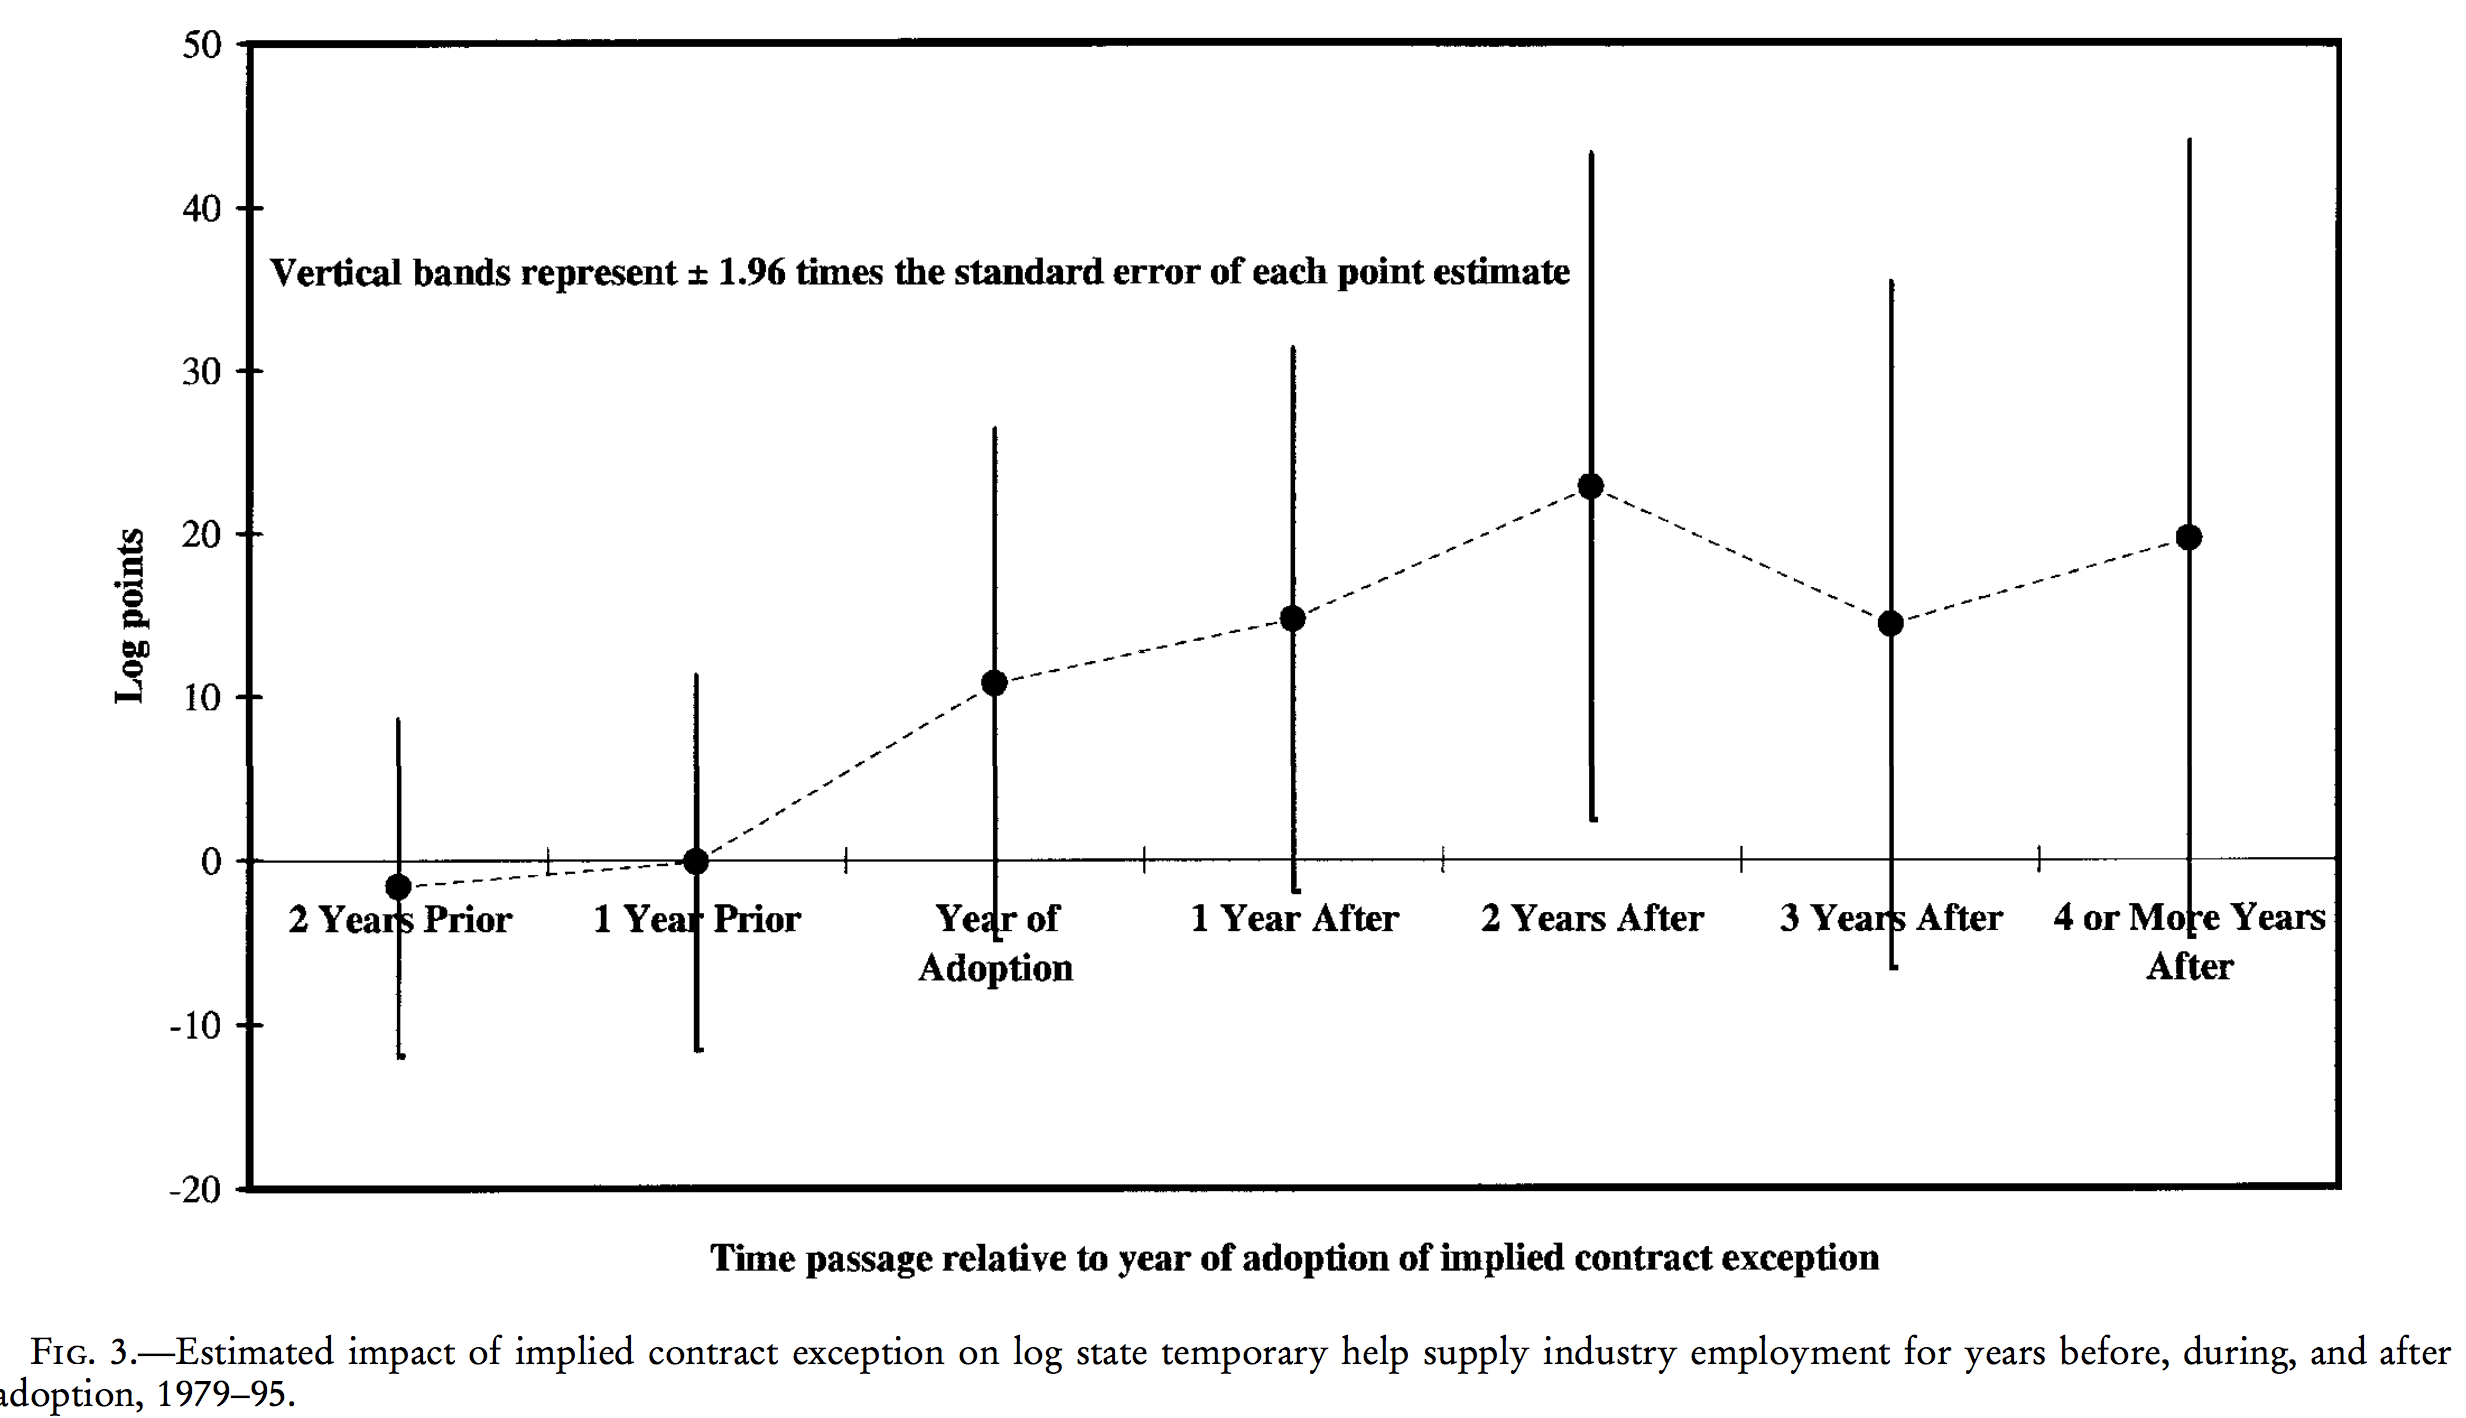
\includegraphics{../Images/autor_fig.png}

\end{frame}

\begin{frame}{Goals for excercise \#2}
\protect\hypertarget{goals-for-excercise-2}{}

\textbf{Primary Goals:}\\
1 - Demonstrate how the \textbf{entire workflow} of a study can fit into
a DD.\\
2 - Show how to add options to the header.\\
3 - Demonstrate how a DD make code readable to non-coders.

\pause

\textbf{Secondary Goal:}\\
1 - Expose you to some R programming.

\end{frame}

\begin{frame}[fragile]{Instructions to get started with excercise \#2:}
\protect\hypertarget{instructions-to-get-started-with-excercise-2}{}

1 - Create a new blank \texttt{.Rmd} file (steps 1 - 3 in from previous
ex.) 2 - Save it as \texttt{/3-dynamicdocs/Figure\ 5-2-4.Rmd}\\
3 - Look at
\href{https://github.com/vikjam/mostly-harmless-replication/blob/master/05\%20Fixed\%20Effects\%2C\%20DD\%20and\%20Panel\%20Data/Figure\%205-2-4.r}{this
code} behind figure 5.2.4.\\
4 - Start building your own DD to describe what this code does.

We will go step by step using
\texttt{/3-dynamicdocs/Figure\ 5-2-4\_solutions.Rmd} as back-up.

\end{frame}

\begin{frame}[fragile]{Description}
\protect\hypertarget{description}{}

\begin{itemize}
\item
  Begin a new section (\texttt{\#\#}), titled ``Description''
\item
  Write a brief description of our goal in the DD.
\item
  You might want to insert a reference to the paper:
  \href{http://economics.mit.edu/files/589}{link here}.
\item
  Specific content not so relevant, just refer to ``a treatment'' and
  ``a outcome''.
\end{itemize}

\end{frame}

\begin{frame}[fragile]{Getting the raw data}
\protect\hypertarget{getting-the-raw-data}{}

\begin{itemize}
\tightlist
\item
  Begin a new section (\texttt{\#\#}), titled ``Raw Data''.\\
\item
  Describe what you will do.\\
\item
  Create two code chunks:
\end{itemize}

\begin{verbatim}
```{r download data, eval=FALSE, echo=TRUE, 
warning=FALSE, results='hide', message=FALSE}
here goes the code
```
\end{verbatim}

\end{frame}

\begin{frame}[fragile]{Cleaning the data}
\protect\hypertarget{cleaning-the-data}{}

\begin{itemize}
\tightlist
\item
  Begin a new section (\texttt{\#\#}), titled ``Data Cleaning''.\\
\item
  Describe what you will do:

  \begin{itemize}
  \tightlist
  \item
    Restrict sample to years between 1979 and 1995 (inclusive)\\
  \item
    Guam from the sample (state = 98).\\
  \end{itemize}
\item
  Create one code chunk:\\
\end{itemize}

\begin{verbatim}
```{r data cleaning, echo=TRUE}
here goes the code
```
\end{verbatim}

\begin{itemize}
\tightlist
\item
  Add some description on the data (using dynamic reporting). See
  solutions (Figure \texttt{5-2-4\_solutions.Rmd} line 58) for examples.
\end{itemize}

\end{frame}

\begin{frame}[fragile]{Build the analytic file}
\protect\hypertarget{build-the-analytic-file}{}

\begin{itemize}
\tightlist
\item
  Begin a new section (\texttt{\#\#}), titled ``Build analytic file''.\\
\item
  Describe what you will do.\\
\item
  We need to construct the following variables:

  \begin{itemize}
  \tightlist
  \item
    Log of total employment\\
  \item
    Normalize the year variable to 1978\\
  \end{itemize}
\item
  Insert a new code chunk:
\end{itemize}

\begin{verbatim}
```{r analytic file, echo=TRUE}
here goes the code
```
\end{verbatim}

\end{frame}

\begin{frame}[fragile]{Describe the model to estimate (optional)}
\protect\hypertarget{describe-the-model-to-estimate-optional}{}

\begin{itemize}
\tightlist
\item
  Begin a new section (\texttt{\#\#}), titled ``Define model to
  estimate''.\\
\item
  One line describing what we want to estimate (i.e. ``We want to
  estimate a fixed effect model with lead and lag treatment
  variables'').\\
\item
  A mathematical model that represents the equation to be estimated
  (look at solutions).
\end{itemize}

\end{frame}

\begin{frame}[fragile]{Vizualize the results (optional)}
\protect\hypertarget{vizualize-the-results-optional}{}

\begin{itemize}
\tightlist
\item
  Begin a new section (\texttt{\#\#}), titled ``Vizualize the
  results''.\\
\item
  One line describing what we want to estimate (i.e. ``This estimates
  are then used to create figure 3 of the original paper, which is
  figure 5.2.4 in MHE.'').\\
\end{itemize}

\begin{verbatim}
```{r viz}
here goes the code
```
\end{verbatim}

\end{frame}

\begin{frame}{Practical Excercise \#2}
\protect\hypertarget{practical-excercise-2-1}{}

\begin{itemize}
\tightlist
\item
  Run your version into multiple outputs.\\
\item
  Run the solutions version into multiple outputs.\\
\item
  Compare document with original version of the code.
\end{itemize}

\end{frame}

\begin{frame}[fragile]{Bonus truck: NBER Working Papers!}
\protect\hypertarget{bonus-truck-nber-working-papers}{}

\begin{itemize}
\item
  Remeber the example from yesterday on the half bake analysis of NBER
  papers in github?
\item
  Fork and clone the repo one more time:
  \href{https://github.com/fhoces/nber_trends}{github.com/fhoces/nber\_trends}
\item
  Now knit the \texttt{.Rmd} file instead.
\end{itemize}

\end{frame}

\hypertarget{final-remarks-more-resources}{%
\section{Final Remarks \& More
Resources}\label{final-remarks-more-resources}}

\begin{frame}[fragile]{Final Remarks \& More Resources}
\protect\hypertarget{final-remarks-more-resources-1}{}

\begin{itemize}
\tightlist
\item
  With DD we can achieve a one-click reproducible workflow.
\item
  This is particularly helpful to understand/present results that are
  hard to digest.
\item
  More great examples in the workshop repo (\texttt{x-moredynamicdocs}).
\item
  Want to learn more: \href{https://bookdown.org/}{great free books}
  (can you guess how they were written?)
\end{itemize}

\end{frame}

\end{document}
